


This chapter contains routines for coordinate transformations, special functions and some miscellaneous but useful computations. Routines for special functions can be found elsewhere, however we give some spherical Bessel function routines, because Matlab does not have them, and a collection of routines for different variations of Legendre polynomials and derivatives that are needed for computing spherical wave functions. Finally, miscellaneous routines include things like FFT frequency generation, vectorized solutions for cubic and quartic roots, and simple ways for generating points on a sphere. 


\section{Coordinate Transformations}

Table \ref{tablecoord} contains coordinates transformations between Cartesian, cylindrical, and spherical coordinates and vector fields, \cite{ulaby1999fundamentals}. The routines in Table \ref{tablecoord} overload the built-in Matlab functions of the same names in order to use $\theta$, $\phi$ orderings and definitions consistent with most scattering textbooks (physics convention, rather than mathematics convention which is what Matlab uses).  The same routines transform between either coordinate points or vector fields. For example, transforming Cartesians points $(x,y,z)$ to spherical coordinates $(r,\theta,\phi)$ is done as
\begin{verbatim}
[r, th, phi] = cart2sph(x,y,z)
\end{verbatim}

The vector transforms always needs the coordinates of the input vector field. For example, transforming a Cartesian vector field $(A_x,A_y,A_z)$ located at points $(x,y,z)$ to spherical vector components $(A_r,A_{\theta},A_{\phi})$ is done as
\begin{verbatim}
[Ar, Ath, Aphi] = cart2sph(x,y,z,Ax,Ay,Az)
\end{verbatim}

Input arrays can be any equal size and $\tan^{-1}$ is always computed with \texttt{atan2}. Unit vectors can be created by setting one of the input vector components equal to 1 and the others to 0.  For example, the Cartesian unit vectors at a point $(x,y,z)$ expressed in spherical coordinates are computed as
\begin{verbatim}
[x_r, x_th, x_phi] = cart2sph(x,y,z,1,0,0) 
[y_r, y_th, y_phi] = cart2sph(x,y,z,0,1,0)  
[z_r, z_th, z_phi] = cart2sph(x,y,z,0,0,1) 
\end{verbatim}

\clearpage
\newpage


\bgroup
\def\arraystretch{1.25}
\begin{table}[h]
\caption{Coordinate Transforms}
\begin{center}
\begin{tabular}{|c| l | l |}
\hline
\multicolumn{1}{|c|}{Routine} & \multicolumn{1}{|c|}{Point Transforms} & \multicolumn{1}{|c|}{Vector Field Transforms} \\
\hline
\texttt{cart2cyl} & 
\threearray{\rho}{\sqrt{x^2 + y^2}}{\phi}{\tan^{-1}(y/x)}{z}{z}  & 
\threearray{A_{\rho}}{A_x \cos\phi + A_y\sin\phi}{A_{\phi}}{-A_x\sin\phi + A_y\cos\phi}{A_z}{A_z}  \\
\hline
\texttt{cyl2cart} & 
\threearray{x}{\rho\cos\phi}{y}{\rho\sin\phi}{z}{z} & 
\threearray{A_x}{A_{\rho}\cos\phi - A_{\phi}\sin\phi}{A_y}{A_{\rho}\sin\phi + A_{\phi}\cos\phi}{A_z}{A_z} \\
\hline
\texttt{cart2sph} & 
\threearray{r}{\sqrt{x^2 + y^2 + z^2}}{\theta}{\tan^{-1}(\sqrt{x^2+y^2}/z)}{\phi}{\tan^{-1}(y/x)} & 
\threearray{A_r}{A_x \st\cos\phi + A_y \sin\theta\sin\phi + A_z \cos\theta}{A_{\theta}}{A_x \ct\cos\phi + A_y \cos\theta\sin\phi - A_z \sin\theta}{A_{\phi}}{-A_x\sin\phi + A_y\cos\phi}\\
\hline
\texttt{sph2cart} & 
\threearray{x}{r\st\cos\phi}{y}{r\st\sin\phi}{z}{r\ct} &
\threearray{A_x}{A_r \st\cos\phi + A_{\theta} \ct\cos\phi - A_{\phi} \sin\phi}{A_y}{A_r \st\sin\phi + A_{\theta} \cos\theta\sin\phi + A_{\phi} \cos\phi}{A_z}{A_r\ct - A_{\theta}\st} \\
\hline
\texttt{cyl2sph} & 
\threearray{r}{\sqrt{\rho^2 + z^2}}{\theta}{\tan^{-1}(\rho/z)}{\phi}{\phi} &
\threearray{A_r}{A_{\rho} \st + A_z\ct}{A_{\theta}}{A_{\rho} \ct - A_z\st}{A_{\phi}}{A_{\phi}} \\
\hline
\texttt{sph2cyl} &
\threearray{\rho}{r\st}{\phi}{\phi}{z}{r\ct} & 
\threearray{A_{\rho}}{A_r\st + A_{\theta}\ct}{A_{\phi}}{A_{\phi}}{A_z}{A_r\ct - A_{\theta}\st} \\
\hline
\end{tabular}
\end{center}
\label{tablecoord}
\end{table}
\egroup


\paragraph{Routine \texttt{cart2cyl} }
{\footnotesize
\VerbatimInput{\code/CoordinateTransforms/cart2cyl.m}
}
\clearpage
\newpage
\paragraph{Routine \texttt{cyl2cart} }
{\footnotesize
\VerbatimInput{\code/CoordinateTransforms/cyl2cart.m}
}
\paragraph{Routine \texttt{cart2sph} }
{\footnotesize
\VerbatimInput{\code/CoordinateTransforms/cart2sph.m}
}
\paragraph{Routine \texttt{sph2cart} }
{\footnotesize
\VerbatimInput{\code/CoordinateTransforms/sph2cart.m}
}
\paragraph{Routine \texttt{cyl2sph} }
{\footnotesize
\VerbatimInput{\code/CoordinateTransforms/cyl2sph.m}
}
\paragraph{Routine \texttt{sph2cyl} }
{\footnotesize
\VerbatimInput{\code/CoordinateTransforms/sph2cyl.m}
}
\paragraph{Helper Routine \texttt{checkargs} }
{\footnotesize
\VerbatimInput{\code/CoordinateTransforms/checkargs.m}
}

\clearpage

\section{Spherical Bessel Functions}

\label{sphericalbess}
Matlab does not have built-in routines for spherical Bessel functions. Below are several variants of spherical Bessel functions and derivatives encountered in scattering problems.

%Log derivatives. 

%\bgroup
%\def\arraystretch{3}
%\begin{table}[htdp]
%\caption{default}
%\begin{center}
%\begin{tabular}{|c|c|c|}
%\hline
%Function & Equation & Comments \\
%\hline
%\texttt{jinc(x)}& $\textrm{jinc}(x) = \dfrac{J_1(x)}{x}$ & $\lim_{x\rightarrow0} \textrm{jinc}(x) = \dfrac{1}{2}$ \\
%\hline
%\texttt{sbesselj(n,x)} & $j_n(x) = \sqrt{\dfrac{\pi}{2x}}J_{n+1/2}(x)$ & $\lim_{x\rightarrow0}j_n(x) = \left\{ \begin{array}{c} 1, \quad n=0 \\ 0, \quad n \ge 1\end{array}  \right.$  \\
%\hline
%\end{tabular}
%\end{center}
%\label{default}
%\end{table}
%\egroup

\addtocontents{toc}{\protect\setcounter{tocdepth}{1}}
\subsection{Sombrero function: $\textrm{jinc}(x)$}
\addtocontents{toc}{\protect\setcounter{tocdepth}{2}}

The \textrm{jinc}(x) function, or Sombrero function, is defined:
\begin{equation}
\textrm{jinc}(x) = \dfrac{J_1(x)}{x}
\end{equation}
%
%\noindent where
%\begin{equation}
%\lim_{z\rightarrow0} \textrm{jinc}(z) = \dfrac{1}{2}
%\end{equation}

\noindent where small arguments are computed with the Taylor series 
\eq{ \textrm{jinc}(x) \approx \dfrac{1}{2} - \dfrac{x^2}{16} + O(x^4)}

{\footnotesize
\VerbatimInput{\code/BesselFunctions/jinc.m}
}

%This is slow in Matlab and we'd like to avoid the division.  Start with the series representation for the Bessel function of complex argument
%\eq{J_{\nu}(z) = \left(\dfrac{z}{2}\right)^\nu \sum_{k=0}^{\infty} \dfrac{ (-1)^k \left( \dfrac{z}{2}\right)^{2k} }{ k! \Gamma(\nu + k + 1)}}
%
%Evaluating $\nu =1$, and dividing by $z$, 
%\eq{\textrm{jinc}(z) = \dfrac{1}{2} \sum_{k=0}^{\infty}(-1)^k a_k }
%\eq{a_k = \dfrac{  \left( \dfrac{z}{2}\right)^{2k} }{ k! \Gamma(k + 2)} }
%
%The log transform is used to avoid multiplying and dividing by large and small numbers, facilitate fast recursive of the factorials, and take care of the limit when $z = 0$.  
%\eq{a_k = e^{\ln a_k}}
%
%where, using $\Gamma(n) = (n-1)!$, 
%\ea{\ln a_k &=& 2k (\ln z - \ln 2) - \ln k! - \ln (k + 1)! }
%
%Evaluating at $k+1$, separating a factor of $\ln a_k$, and shifting the index down by 1, we get the recursion for the $k$th term of the series
%\ea{\ln a_{0} &=& 0 \\
%\ln a_{k} &=& \ln a_{k-1} + 2 (\ln z - \ln 2) - \ln k - \ln (k + 1) }
%
%%\ea{\ln a_{k+1} &=& 2(k+1) (\ln z - \ln 2) - \ln (k+1)! - \ln (k + 2)! \\
%%\ &=& 2k (\ln z - \ln 2) + 2 (\ln z - \ln 2) - (\ln k! + \ln (k+1)) - ( \ln (k + 1)!  + \ln (k + 2) ) \\
%%\ &=& \ln a_k + 2 (\ln z - \ln 2) - \ln (k+1) - \ln (k + 2) }
%
%The code is as follows.  

\addtocontents{toc}{\protect\setcounter{tocdepth}{1}}
\subsection{Spherical Bessel function: $j_n(x)$}
\addtocontents{toc}{\protect\setcounter{tocdepth}{2}}

The spherical Bessel function is 

\begin{equation}
j_n(x) = \sqrt{\dfrac{\pi}{2x}}J_{n+1/2}(x)
\end{equation}

\noindent where

\begin{equation}
\lim_{x\rightarrow0}j_n(x) = \left\{ \begin{array}{c} 1 - \dfrac{x^2}{6} + O(x^4) \quad n=0 \\ 0, \quad n \ge 1\end{array}  \right.
\end{equation}

The routine \texttt{sbesselj} returns the spherical Bessel function for matching arrays of $n$ and $x$ in the format of \texttt{besselj}. It uses the Taylor series near $x = 0$ for $n=0$, and substitutes 0 when $x=0$ for $n>1$.  

{\footnotesize
\VerbatimInput{\code/BesselFunctions/sbesselj.m}
}

\addtocontents{toc}{\protect\setcounter{tocdepth}{1}}
\subsection{Spherical Bessel function: $j_n(x)/x$}
\addtocontents{toc}{\protect\setcounter{tocdepth}{2}}


This variant of the spherical Bessel function has $j_n(x)$ divided by $x$: 
\begin{equation}
\dfrac{j_n(x)}{x} = \dfrac{1}{x^{3/2}}\sqrt{\dfrac{\pi}{2}}J_{n+1/2}(x)
\end{equation}

\noindent where
\begin{equation}
\lim_{x\rightarrow0}j_n(x) = \left\{ \begin{array}{c} \infty, \quad n=0 \\ \dfrac{1}{3} - \dfrac{x^2}{30} + O(x^4), \quad n = 1 \\ 0, \quad n \ge 2\end{array}  \right.
\end{equation}

This is computed in the routine \texttt{sbesselj2}, which takes the same inputs as \texttt{sbesselj}.  We let the routine return \texttt{Inf} for $x=0$ when $n=0$.  This variant is found in electromagnetic scattering when usually the monopole term ($n=0$) is not needed.

{\footnotesize
\VerbatimInput{\code/BesselFunctions/sbesselj2.m}
}

\addtocontents{toc}{\protect\setcounter{tocdepth}{1}}
\subsection{Spherical Bessel function derivative: $j_n'(x)$}
\addtocontents{toc}{\protect\setcounter{tocdepth}{2}}

The derivative of the spherical Bessel function with respect to $x$ is given by the recurrence relation
\begin{equation}
j_n'(x) = -j_{n+1}(x) + \dfrac{n}{x}j_n(x)
\end{equation}

This is computed in \texttt{sbesseljp} with \texttt{sbesselj} and \texttt{sbesselj2}, which takes care of $x=0$. 

{\footnotesize
\VerbatimInput{\code/BesselFunctions/sbesseljp.m}
}

\clearpage
\addtocontents{toc}{\protect\setcounter{tocdepth}{1}}
\subsection{Spherical Bessel function derivative: $[xj_n(x)]'$}
\addtocontents{toc}{\protect\setcounter{tocdepth}{2}}

This variant occurs often enough in scattering to have its own function, \texttt{sbesseljp2}, 
\ea{[xj_n(x)]' &=& j_n(x) + x j'_n(x) \\
\ &=&  (1+n)j_n(x) - x j_{n+1}(x)}

This variant is found in the Mie scattering solution for spheres.

{\footnotesize
\VerbatimInput{\code/BesselFunctions/sbesseljp2.m}
}


\addtocontents{toc}{\protect\setcounter{tocdepth}{1}}
\subsection{Spherical Hankel function: $h_n^{(1)}(x)$}
\addtocontents{toc}{\protect\setcounter{tocdepth}{2}}

The spherical Hankel function is given by 
\begin{equation}
h_n^{(1)}(x) = \sqrt{\dfrac{\pi}{2x}}H_{n+1/2}(x)
\end{equation}

This is always irregular at the origin, and computed in the routine \texttt{sbesselh}

{\footnotesize
\VerbatimInput{\code/BesselFunctions/sbesselh.m}
}

\addtocontents{toc}{\protect\setcounter{tocdepth}{1}}
\subsection{Spherical Hankel function derivative: ${h'}_n^{(1)}(x)$}
\addtocontents{toc}{\protect\setcounter{tocdepth}{2}}

The spherical Hankel derivative is computed in the routine \texttt{sbesselhp}
\begin{equation}
{h'}_n^{(1)}(x) = -h_{n+1}^{(1)}(x) + \dfrac{n}{x}h_n^{(1)}(x)
\end{equation}


{\footnotesize
\VerbatimInput{\code/BesselFunctions/sbesselhp.m}
}

\addtocontents{toc}{\protect\setcounter{tocdepth}{1}}
\subsection{Spherical Hankel function derivative: $[xh_n^{(1)}(x)]'$}
\addtocontents{toc}{\protect\setcounter{tocdepth}{2}}

Similar to before, this variant is computed in the routine \texttt{sbesselhp2}
\ea{[xh_n^{(1)}(x)]' &=& h_n^{(1)}(x) + x {h'}_n^{(1)}(x) \\
\ &=&  (1+n)h_n^{(1)}(x) - x h_{n+1}^{(1)}(x)}

This variant is found in the Mie scattering solution for spheres.


{\footnotesize
\VerbatimInput{\code/BesselFunctions/sbesselhp2.m}
}


\clearpage

\section{Legendre Polynomials}

The routines in this section compute Legendre polynomials,  normalized associated Legendre polynomials and their derivatives in formats useful to scattering. Associated Legendre polynomials are computed at both positive and negative $m$ and automatically include the Condon-Shortley phase.  

\addtocontents{toc}{\protect\setcounter{tocdepth}{1}}
\subsection{Legendre Polynomials, $P_l(x)$}
\addtocontents{toc}{\protect\setcounter{tocdepth}{2}}


The Legendre polynomials satisfy the equation
\begin{equation}
\dfrac{d}{dx} \left[ (1-x^2)\dfrac{d}{dx}P_l(x)\right] + l(l+1)P_l(x) = 0
\end{equation}

for $-1 \le x \le 1$, with the following recurrence relation
\begin{equation}
(l+1)P_{l+1}(x) = (2l+1)xP_l(x) - lP_{l-1}(x) \label{plrec}
\end{equation}

The routine \texttt{legendrePl} returns $P_l(x)$ on a 2D array with degrees $0$ to $L$ along rows and evaluation points along columns.  


{\footnotesize
\VerbatimInput{\code/LegendrePolynomials/legendrePl.m}
}

\clearpage
\addtocontents{toc}{\protect\setcounter{tocdepth}{1}}
\subsection{Legendre Polynomial Derivative, $d/dx P_l(x)$}
\addtocontents{toc}{\protect\setcounter{tocdepth}{2}}

The derivative of the Legendre polynomials satisfies either of the following recurrence relations
\begin{equation}
\dfrac{x^2-1}{l}\dfrac{d}{dx}P_l(x) = xP_l(x) - P_{l-1}(x)
\end{equation}

\begin{equation}
(2l+1)P_l(x) = \dfrac{d}{dx}(P_{l+1}(x) - P_{l-1}(x))
\end{equation}

The first has a divide by zero when $x$ is 1 or -1.  Rearranging the second equation we get following recurrence 
\begin{equation}
\dfrac{d}{dx}P_{l+1}(x) = (2l+1)P_l(x) + \dfrac{d}{dx} P_{l-1}(x)
\end{equation}

\noindent which is safe on $x=[-1, 1]$.  Initial conditions are the special cases $P'_0(x) = 0$ and $P'_1(x) = 1$, and the derivative has the feature that $P'_l(1) = l(l+1)/2$.  The routine \texttt{legendrePlp} is like \texttt{legendrePl}: it returns $d/dx P_l(x)$ on a 2D array with degrees $0$ to $L$ along rows and evaluation points along columns.  

{\footnotesize
\VerbatimInput{\code/LegendrePolynomials/legendrePlp.m}
}

\clearpage
\addtocontents{toc}{\protect\setcounter{tocdepth}{1}}
\subsection{Normalized Associated Legendre Polynomials, $\widetilde{P}_l^m(x)$}
\addtocontents{toc}{\protect\setcounter{tocdepth}{2}}


The associated Legendre polynomials, $P_l^m(x)$, are given by
\begin{equation}
P_l^m(x) = \dfrac{(-1)^m}{2^l l!} (1-x^2)^{m/2} \dfrac{d^{l+m}}{dx^{l+m}} (x^2 - 1)^l \label{plm}
\end{equation}

\noindent for integers $l$ and $m$ such that $l \ge 0$ and $-l \le m \le l$.  The Condon-Shortley phase is included in the definition of the associated Legendre polynomials. The following identity relates positive and negative $m$
\begin{equation}
P_l^{-m}(x) = (-1)^m \dfrac{(l-m)!}{(l+m)!} P_l^m(x)\
\label{eq2}
\end{equation}

The normalized associated Legendre polynomials $\widetilde P_l^m(x)$ are recommended for scattering computations because they avoid direct computation of factorials. These are given by
\begin{equation}
\widetilde P_l^m(x) = \sqrt{\dfrac{(l + \frac{1}{2})(l-m)!}{(l+m)!}} P_l^m(x) \label{plmnorm}
\end{equation}

\noindent where
\begin{equation}
\widetilde P_l^{-m}(x) = (-1)^m \widetilde{P}_l^m(x)
\end{equation}

The routine \texttt{Plm} returns the normalized associated Legendre polynomials for $l=0,...,L$, all $\pm m$, linearly indexed (see Chapter \ref{chap:wavefunctions} on linear indexing). The result is returned with harmonics indexed along rows, and evaluation points along columns. It calls Matlab's \texttt{legendre} with the \texttt{'norm'} option, which returns $m = 0,...,l$ and an extra factor of $(-1)^m$. \texttt{Plm} takes out the extra $(-1)^m$ from Matlab's normalization so that the one factor of $(-1)^m$ in \eqref{plm} remains. %Use the switch \texttt{'scalar'} to include the $(l,m) = (0,0)$ term. The total number of harmonics is $N = L^2 + 2L$ or $N = L^2 + 2L + 1$ for scalar.

{\footnotesize
\VerbatimInput{\code/LegendrePolynomials/Plm.m}
}



%
%\subsection{Normalized Associated Legendre Polynomials Derivative, $d/dx\widetilde{P}_l^m(x)$}
%
%The derivative of the associated Legendre polynomials has several recurrence relations that are given in terms of the non-differentiated functions, but they all have the problem of divide by zero at $\pm1$. A mixed recurrence on $l$ can be derived starting with the unnormalized recurrence
%\eq{(l-m+1)P_{l+1}^m(x) = (2l+1)xP_l^m(x) - (l+m)P_{l-1}^m(x)}
%
%and differentiating, which gives
%\eq{(l-m+1)\dfrac{d}{dx}P_{l+1}^m(x) =  (2l+1)\left( P_l^m(x) +  x\dfrac{d}{dx}P_l^m(x)\right)- (l+m)\dfrac{d}{dx}P_{l-1}^m(x) \label{dpplus}}
%
%Substituting the expression for the normalized Legendre polynomials into \eqref{dpplus} and simplifying
%%
%%\eq{\sqrt{\dfrac{(l+m)!}{(l + \frac{1}{2})(l-m)!}} \widetilde P_l^m(x) =  P_l^m(x)}
%%
%%\ea{(l-m+1)\sqrt{\dfrac{(l+1+m)!}{(l +1+ \frac{1}{2})(l+1-m)!}} \dfrac{d}{dx}\widetilde P_{l+1}^m(x) &=&  (2l+1)\sqrt{\dfrac{(l+m)!}{(l + \frac{1}{2})(l-m)!}} \left( \widetilde P_l^m(x)   +  x\dfrac{d}{dx}\widetilde P_l^m(x)\right)\\
%%\ &\ & - (l+m)\sqrt{\dfrac{(l-1+m)!}{(l -1 + \frac{1}{2})(l-1-m)!}} \dfrac{d}{dx}\widetilde P_{l-1}^m(x)  \label{dpplus} }
%%
%%\ea{(l-m+1)\sqrt{\dfrac{(l+1+m)(l+m)}{(l +1+ \frac{1}{2})(l+1-m)(l-m)}} \dfrac{d}{dx}\widetilde P_{l+1}^m(x) &=&  (2l+1)\sqrt{\dfrac{(l+m)}{(l + \frac{1}{2})(l-m)}} \left( \widetilde P_l^m(x)   +  x\dfrac{d}{dx}\widetilde P_l^m(x)\right)\\
%%\ &\ & - (l+m)\sqrt{\dfrac{1}{(l -1 + \frac{1}{2})}} \dfrac{d}{dx}\widetilde P_{l-1}^m(x)  \label{dpplus} }
%
%\ea{  \dfrac{d}{dx}\widetilde P_{l+1}^m(x) &=&   a_{l,m} \left( \widetilde P_l^m(x)   +  x\dfrac{d}{dx}\widetilde P_l^m(x)\right) -  b_{l,m} \dfrac{d}{dx}\widetilde P_{l-1}^m(x)  }
%%
%%\ea{a_{l,m} &=& \dfrac{1}{(l-m+1)}\sqrt{\dfrac{(l +1+ \frac{1}{2})(l+1-m)(l-m)}{(l+1+m)(l+m)}}  (2l+1)\sqrt{\dfrac{(l+m)}{(l + \frac{1}{2})(l-m)}} \\
%%b_{l,m} &=&  \dfrac{1}{(l-m+1)}\sqrt{\dfrac{(l +1+ \frac{1}{2})(l+1-m)(l-m)}{(l+1+m)(l+m)}}(l+m)\sqrt{\dfrac{1}{(l -1 + \frac{1}{2})}}}
%
%\ea{a_{l,m} &=&  2 \sqrt{\dfrac{(l + \frac{3}{2})(l + \frac{1}{2}) }{(l-m+1)(l+m+1) }}   \\
%b_{l,m} &=&   \sqrt{\dfrac{(l +\frac{3}{2}) (l-m)(l+m)}{(l - \frac{1}{2})(l-m+1)(l+m+1) }} }
%
%This is initialized along the $m = l$ diagonal with 
%\eq{ \dfrac{d}{dx} \widetilde P_{0}^0(x) = 0}
%\eq{  \dfrac{d}{dx} \widetilde P_{l+1}^l(x) = \sqrt{\dfrac{(2l+1)(l + \frac{3}{2})}{(l + \frac{1}{2})}} \left(\widetilde P_l^l(x) + x \dfrac{d}{dx} \widetilde P_{l}^l(x) \right)}
%
%which comes from differentiating $P_{l+1}^l (x) = x(2l+1)P_l^l(x)$ and normalizating. 
%
%%\eq{\sqrt{\dfrac{(l+m)!}{(l + \frac{1}{2})(l-m)!}} \widetilde P_l^m(x) =  P_l^m(x)}
%
%
%%\eq{ \sqrt{\dfrac{(l+1+m)!}{(l + 1 + \frac{1}{2})(l+1-m)!}} \widetilde P_{l+1}^m(x) = x(2l+1) \sqrt{\dfrac{(l+m)!}{(l + \frac{1}{2})(l-m)!}} \widetilde P_l^m(x) }
%%
%%\eq{ \sqrt{\dfrac{(l+1+l)!}{(l + 1 + \frac{1}{2})}} \widetilde P_{l+1}^l(x) = x(2l+1) \sqrt{\dfrac{(l+l)!}{(l + \frac{1}{2})}} \widetilde P_l^l(x) }
%%
%%\eq{ \sqrt{\dfrac{(2l+1)}{(l + 1 + \frac{1}{2})}} \widetilde P_{l+1}^l(x) = x(2l+1) \sqrt{\dfrac{1}{(l + \frac{1}{2})}} \widetilde P_l^l(x) }
%
%%\eq{  \widetilde P_{l+1}^l(x) = c_{l,m} x  \widetilde P_l^l(x) }
%
%
%This recurrence requires both degrees less than or equal to $l$.  This is given by the routine \texttt{Plmp}, and has the same structure as \texttt{Plm}.   
%
%{\footnotesize
%\VerbatimInput{\code/LegendrePolynomials/Plmp.m}
%}
%
%

\addtocontents{toc}{\protect\setcounter{tocdepth}{1}}
\subsection{Normalized Associated Legendre Polynomials Derivative, $d/dx\widetilde{P}_l^m(x)$}
\addtocontents{toc}{\protect\setcounter{tocdepth}{2}}


The derivative of the normalized associated Legendre polynomials is found by substituting \eqref{plmnorm} into the following non-normalized recurrence relation for the associated Legendre polynomial derivative:
\eq{(x^2-1) \dfrac{d}{dx} P_l^m(x) = lx P_l^m(x) - (l+m)P_{l-1}^m(x)}

which gives
\begin{equation}
\dfrac{d}{dx}\widetilde P_l^m(x) = \dfrac{1}{x^2-1}\left( lx \widetilde P_l^m(x) - \sqrt{\dfrac{(l+1/2)}{(l-1/2)}}\sqrt{(l+m)(l-m)} \widetilde P_{l-1}^m(x)\right)
\end{equation}

This recurrence only requires $\widetilde P_l^m(x)$ to be computed at degrees less than or equal to $l$.  This is computed by the routine \texttt{Plmp}, and has the same structure as \texttt{Plm}, which returns $l=0,...,L$, all $\pm m$, linearly indexed (see Chapter \ref{chap:wavefunctions}). This version is not suitable at the end points $x = [-1, 1]$. In fact, the difficultly of computing the derivative of the associated Legendre polynomials at the end-points is well-known, and other routines can be found elsewhere. However, we use this routine in scattering problems when the poles do not need to be sampled, for example, when using Gauss-Legendre quadrature as the basis for spherical harmonic transforms (see Chapter \ref{chap:fmm}). 

{\footnotesize
\VerbatimInput{\code/LegendrePolynomials/Plmp.m}
}

\clearpage
\addtocontents{toc}{\protect\setcounter{tocdepth}{1}}
\subsection{Normalized Associated Legendre Polynomials, $m\widetilde{P}_l^m(\cos\theta)/\sin\theta $}
\addtocontents{toc}{\protect\setcounter{tocdepth}{2}}


The variant $m\widetilde{P}_l^m(\cos\theta)/\sin\theta $ is needed for vector wave functions. Numerically, direct division by $\sin\theta$ is a problem at the poles, however, analytically, dividing by $\sin\theta$ is harmless because $P_l^m(\cos\theta) \sim \sin^m\theta$.  With the right recurrence relation, it can be computed directly.  Start with the following unnormalized recurrence relation
\begin{equation}
\dfrac{m}{\sin\theta}P_l^m(\cos\theta) = -\dfrac{1}{2}\left(P_{l-1}^{m+1}(\cos\theta) + (l+m-1)(l+m)P_{l-1}^{m-1}(\cos\theta) \right) 
\end{equation}

Then substituting \eqref{plmnorm} and canceling like factorials
\begin{eqnarray}
\dfrac{m}{\sin\theta}\widetilde P_l^m(\cos\theta)& =& \dfrac{1}{2}\sqrt{\dfrac{l-\frac{1}{2}}{l+\frac{1}{2}}}\left(\sqrt{(l-m)(l-m-1)}\widetilde P_{l-1}^{m+1}(\cos\theta)\right. \nonumber \\
\ & \ & +\left. \sqrt{(l+m)(l+m-1)}\widetilde P_{l-1}^{m-1}(\cos\theta) \right) 
\end{eqnarray}

This is computed by the routine \texttt{mPlmsin}, and has similar structure to \texttt{Plm}.  It returns degrees $l = 1,..,L$, all $m$, linearly indexed along rows with evaluation points along columns.  We exclude the monopole because this variant is only used for vector wave functions. It uses the initial condition
\begin{equation}
\dfrac{(1)}{\sin\theta}\widetilde P_1^1(\cos\theta) = \sqrt{\dfrac{3}{4}}
\end{equation}

Technically this initial condition should have a negative sign. However, we iterate on the output of the Matlab's \texttt{legendre}, which has an extra negative sign. Therefore, we adjust the negative signs at the end of the routine so that the outputs will match a direct computation of the quantity $m\widetilde{P}_l^m(\cos\theta)/\sin\theta $ when using \texttt{Plm}. 

{\footnotesize
\VerbatimInput{\code/LegendrePolynomials/mPlmsin.m}
}


\addtocontents{toc}{\protect\setcounter{tocdepth}{1}}
\subsection{Normalized Associated Legendre Polynomials Derivative, $d/d\theta\widetilde{P}_l^m(\cos\theta)$}
\addtocontents{toc}{\protect\setcounter{tocdepth}{2}}


The variant $d/d\theta\widetilde{P}_l^m(\cos\theta)$ is the derivative of the normalized associated Legendre polynomials with respect to $\theta$ when the argument is $\cos\theta$.  Start with the recurrence relation for unnormalized Legendre polynomials 
\begin{eqnarray}
\dfrac{d}{d\theta}P_l^m(\cos\theta) &= &-\sin\theta \dfrac{d}{d\cos\theta}P_l^m(\cos\theta)  \\
\ &=& -\dfrac{1}{2}\left((l+m)(l-m+1)P_l^{m-1}(\cos\theta) -P_l^{m+1}(\cos\theta)\right) 
\end{eqnarray}

Substituting the expression for the normalized Legendre polynomials and canceling like factorials 
\eq{
\dfrac{d}{d\theta}\widetilde P_l^m(\cos\theta) = \dfrac{1}{2}\left(\sqrt{(l+m)(l-m+1)}\widetilde P_l^{m-1}(\cos\theta) - \sqrt{(l-m)(l+m+1)}\widetilde P_l^{m+1}(\cos\theta)\right)  
}
%
%\begin{eqnarray}
%\dfrac{d}{d\theta}\widetilde P_l^m(\cos\theta) &=& \dfrac{1}{2}\left(\sqrt{(l+m)(l-m+1)}\widetilde P_l^{m-1}(\cos\theta)\right. \nonumber \\
%\ & \ & -\left. \sqrt{(l-m)(l+m+1)}\widetilde P_l^{m+1}(\cos\theta)\right)  
%\end{eqnarray}

This recurrence only requires degrees equal to $l$.  This is given by the routine \texttt{Plmp2}, and has similar structure to \texttt{Plm}.  It returns degrees $l = 1,..,L$, all $m$, linearly indexed in rows and evaluation points along columns.  We exclude the monopole because this variant is used for vector wave functions, and because the derivative for $(l,m) = (0,0)$ is zero.  It uses the initial condition 
\begin{equation}
\dfrac{d}{d\theta}\widetilde{P}_l^0(\cos\theta) = -\sqrt{l(l+1)}\widetilde{P}_l^1(\cos\theta) 
\end{equation}

{\footnotesize
\VerbatimInput{\code/LegendrePolynomials/Plmp2.m}
}

\clearpage


\section{Miscellaneous}

\subsection{FFT Frequency}

It is surprisingly hard to remember the frequency samples that match the unshifted two-sided discrete Fast Fourier Transform (FFT) for odd or even length signals. Let $f_s$ be the sample frequency and $N$ be the number of points, then the discrete frequencies of the FFT are:

$N$ even:
\begin{equation}
f[k] = \dfrac{f_s}{N}\begin{cases}
    k,& k = 0,..., \dfrac{N}{2} - 1\\
    k-N, & k = \dfrac{N}{2}, ..., N-1 
\end{cases}
\end{equation}

$N$ odd:
\begin{equation}
f[k] = \dfrac{f_s}{N}\begin{cases}
    k,& k = 0,..., \dfrac{N-1}{2} \\
    k-N, & k = \dfrac{N+1}{2}, ..., N-1 
\end{cases}
\end{equation}

The routine \texttt{fftfreq} takes as input the sampling rate, $f_s$, and number of points, $N$, and returns the discrete frequencies $f[k]$ that correspond to the unshifted two-sided FFT of odd or even $N$.

{\footnotesize
\VerbatimInput{\code/Misc/fftfreq.m}
}



\subsection{Phase wrapping}

Phase wrapping is easily done with $\angle \exp(i\phi)$, but there is a fun variation that uses nearest integer rounding written in terms of elementary functions: 
\begin{eqnarray}
\Phi(\phi) & = & \phi - 2\pi\left[\dfrac{\phi}{2\pi} \right] \\
\ & = & -2\arctan\cot\left(\dfrac{\phi}{2} + \dfrac{\pi}{2}\right) 
\end{eqnarray} 

\noindent where $[\cdot ]$ means round to the nearest integer so that $-\pi \le \Phi \le \pi$. %In principle, this can be differentiated away from the wrap points.  

{\footnotesize
\VerbatimInput{\code/Misc/wrap.m}
}

%http://functions.wolfram.com/IntegerFunctions/Round/introductions/FloorRelated/ShowAll.html

%
%\subsection{Complex Standard Normal Distribution}
%
%The complex standard normal distribution is defined
%
%\begin{equation}
%\gamma = \dfrac{1}{\sqrt{2}}\left( \mathcal{N}(0,1) + i \mathcal{N}(0,1)\right)
%\end{equation}
%
%\noindent where $\mathcal{N}(0,1)$ is a normal distribution with zero mean and unit variance.  This is used to add noise to complex signals or to seed power spectral densities (PSD) in the frequency domain. For the later, we require $\gamma$ to have conjugate symmetry if the inverse Fourier transform is to yield a real valued signal. Because the Fourier transform of a Gaussian random variable is also Gaussian, a lazy way to ensure conjugate symmetry is to take the DFT of an array loaded with the real valued standard normal. However, a faster and more practical way to generate a signal from a PSD is simply to seed the PSD with the complex standard normal, without conjugate symmetry, and take the real part after the IFFT.  
%
%The routines \texttt{gamman} and \texttt{gammanw} return the complex standard normal and frequency domain complex standard normal, respectively, for an arbitrary number of dimensions of sizes $N_1$, $N_2$, etc.  The frequency domain version is computed with the DFT, which requires division by the dimension lengths.  It can be verified that for both the real and imaginary parts of each functions that the mean and variance are $0$ and $1/\sqrt{2}$, respectively.  In \texttt{gammanw}, we set the DC component to zero to guarantee zero mean.  
%
%{\footnotesize
%\VerbatimInput{\code/Misc/gamman.m}
%}
%
%{\footnotesize
%\VerbatimInput{\code/Misc/gammanw.m}
%}

\clearpage
\newpage
\subsection{Cubic Roots}

The roots of a cubic polynomial are known analytically. Let the cubic be written
\eq{a x^3 + b x^2 + c x + d = 0}

and define
\ea{w &=& -\dfrac{b}{3a} \\
Q &=& \dfrac{3ac - b^2}{9a^2} \\
R&=& \dfrac{9abc - 27a^2d - 2b^3}{54a^3} \\
D &=& Q^3 + R^2}

When $D\ge0$, there is one real root and two complex conjugate roots. For this case, define
\ea{S &=& \sqrt[3]{R + \sqrt{D}} \\
T &=&  \sqrt[3]{R - \sqrt{D}} }

When $D < 0$, there are three real roots and the following is used
\ea{S &=& \sqrt[3]{\rho}e^{i \theta/3} \\
T &=&  \sqrt[3]{\rho}e^{-i \theta/3} \\
\rho &=& \sqrt{-Q^3} \\
\theta &=& \arccos\left(\dfrac{R}{\rho}\right)}

In all instances, the positive roots of $\sqrt[3]{}$ and $\sqrt{}$ are used. The roots of the cubic are then given by 
\ea{x_1 &=& w + S + T \\
x_2 &=& w -\dfrac{1}{2}(S +T) + i\dfrac{\sqrt{3}}{2}(S-T) \\
x_3 &=& w -\dfrac{1}{2}(S +T) - i\dfrac{\sqrt{3}}{2}(S-T) }

\noindent where $x_1$ is always real.

The routine \texttt{cubicroots} is a vectorized implementation of the solution above that computes the roots of multiple cubic polynomials simultaneously. Coefficient arrays can be any size. When \texttt{nargout == 1}, the routine returns the guaranteed real root $x_1$. The key difference between this routine and Matlab's \texttt{roots} is that \texttt{roots} is not vectorized and only solves one polynomial at a time, otherwise, the two routines produce the same solutions.

{\footnotesize
\VerbatimInput{\code/Misc/cubicroots.m}
}

\subsection{Quartic Roots}

Like the cubic, the roots of a quartic polynomial are known analytically, \cite{weisstein_quartic}.  Let the quartic be written 
\eq{a x^4 + b x^3 + c x^2 + d x + e = 0}

This is put in standard form by dividing the leading coefficient
\eq{x^4 + a_3 x^3 + a_2 x^2 + a_1 x + a_0 = 0}

\noindent where $a_3 = b/a$, $a_2 = c/a$, $a_1 = d/a$ and $a_0 = e/a$.  This has resolvent cubic
\eq{y^3 - a_2y^2 + (a_1a_3-4a_0) y + (4 a_2 a_0 - a_1^2-a_3^2 a_0) = 0 \label{resolvecube}}

If $y_1$ is any real root of \eqref{resolvecube} (there is always at least one), then the roots of the quartic are given by 
\ea{x_{1,2} &=& w + \dfrac{1}{2}R \pm \dfrac{1}{2}D \\
x_{3,4} &=& w - \dfrac{1}{2}R \pm \dfrac{1}{2}E }

\noindent where
\ea{ D &=& \begin{cases}  \sqrt{T - R^2 + \dfrac{U}{R}}, \quad R\ne 0 \\ \sqrt{T + V},\quad \quad \quad \quad R = 0 \end{cases} \\
E &=& \begin{cases}  \sqrt{T - R^2 - \dfrac{U}{R}}, \quad R\ne 0 \\ \sqrt{T - V}, \quad \quad \quad \quad R = 0 \end{cases} }

and
\ea{w &=& -\dfrac{1}{4} a_3 \\
R &=& \sqrt{\dfrac{a_3^2}{4} - a_2 + y_1} \\
T &=& \dfrac{3 a_3^2}{4} - 2 a_2\\
U &=& \dfrac{4a_3a_2-8a_1-a_3^3}{4} \\
V &=& 2 \sqrt{y_1^2 - 4 a_0} }


The routine \texttt{quarticroots} is a vectorized implementation of the solution above that computes the roots of multiple quartic polynomials simultaneously. Coefficient arrays can be any size. The real cubic root, $y_1$, comes from \texttt{cubicroots}. Again, Matlab's \texttt{roots} only solves one polynomial at a time, otherwise the two routines produce the same solutions.

{\footnotesize
\VerbatimInput{\code/Misc/quarticroots.m}
}

\clearpage
\newpage
\subsection{Uniform Points on a Sphere}

A quick approximation of uniform points on a sphere is based on the disco ball. Points are distributed mostly evenly at discrete latitudes centered on a prime meridian. This avoids crowding at the poles that happens with uniform sampling in spherical coordinates. Specifically, the number of lines of latitude is chosen which are divided equally between $\theta = [0, \pi]$, then each circle of constant latitude is divided by the latitude spacing as many times as it will go.

The routine \texttt{discoball} takes as input the number of latitude lines \texttt{nlat} and returns the spherical coordinates of the points $(\theta,\phi)$.  

\begin{figure}[H]
\centering
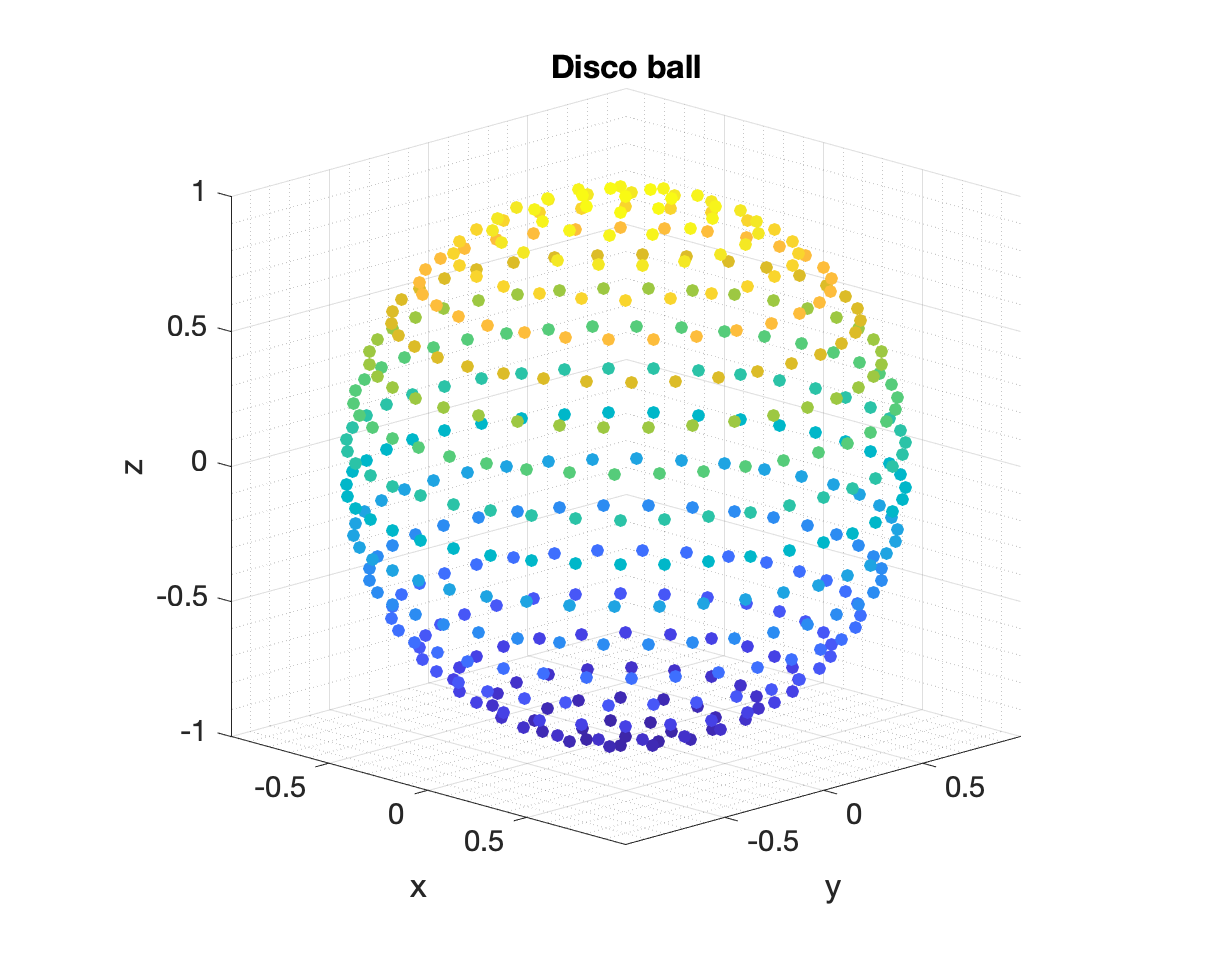
\includegraphics[width=3.5in]{Utilities/Figures/discoball}
\caption{Disco ball approximation for uniform points on a sphere}
\end{figure}

{\footnotesize
\VerbatimInput{\code/Misc/discoball.m}
}

\clearpage
\newpage

\subsection{Uniformly Random Points on a Sphere}

To create a set of points that are uniformly random over the unit sphere, it is not correct to draw from a uniformly random distribution of spherical angles $(\theta,\phi)$, because this leads to crowding at the poles.  Instead, the following transformation is used, \cite{randsphere}, 
\begin{eqnarray}
\phi &=& 2\pi U(0,1) \\
\theta &=& \arccos(2V(0,1)-1)
\end{eqnarray}

\noindent where $U(0,1)$ and $V(0,1)$ are uniform random variables from $[0,1]$.  

The routine \texttt{randsphere} takes as input the total number of points, $N$, and returns the spherical $(\theta,\phi)$ coordinates of the points.  

\begin{figure}[H]
\centering
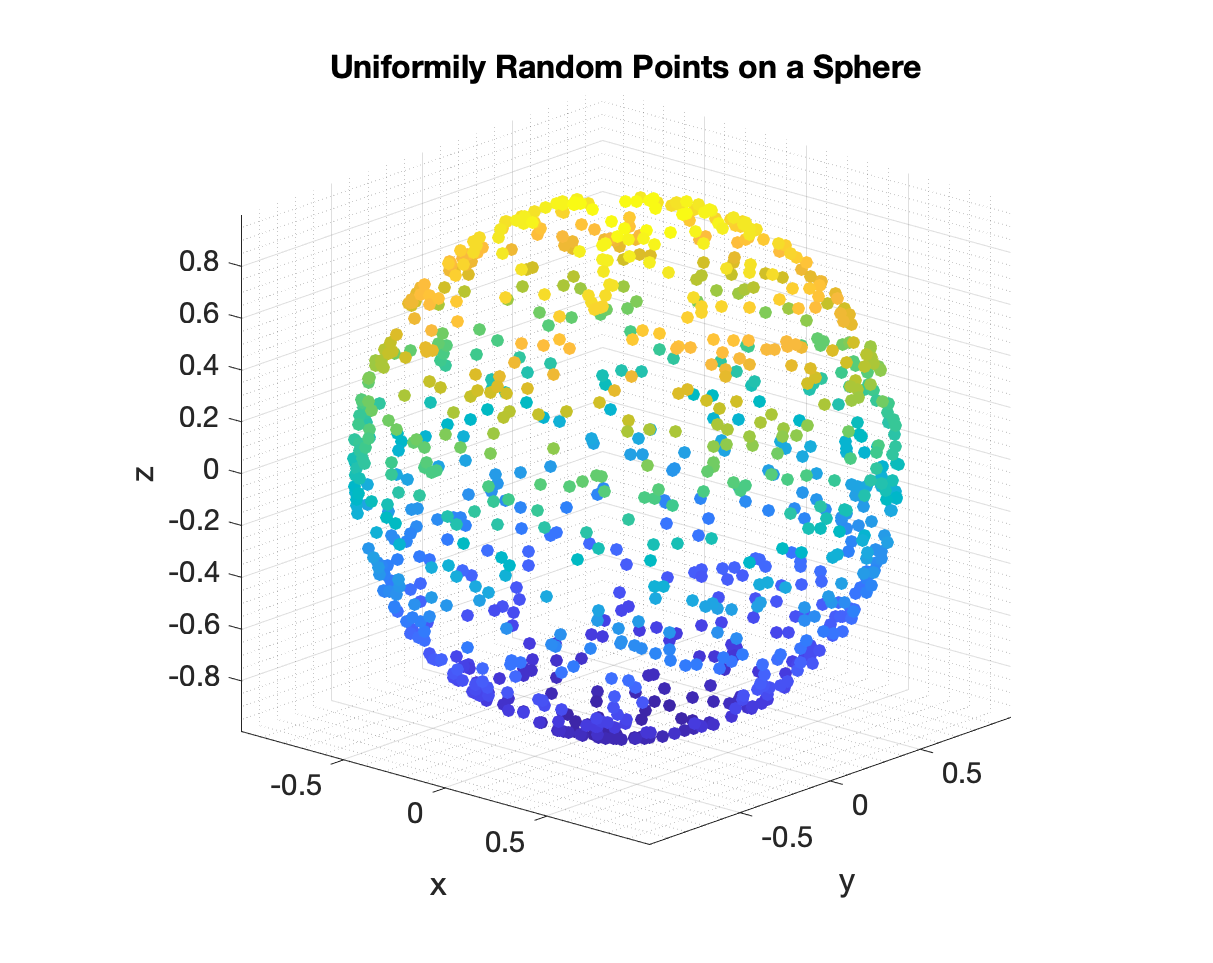
\includegraphics[width=3.5in]{Utilities/Figures/uniformrand}
\caption{Uniformly random points on a sphere, $N = 1000$. }
\end{figure}

{\footnotesize
\VerbatimInput{\code/Misc/randsphere.m}
}

%
%\subsection{$\log_b(x)$}
%
%Matlab doesn't have this.
%
%\begin{equation}
%\log_b(x) = \log(x)/\log(b)
%\end{equation}
%
%{\footnotesize
%\VerbatimInput{\code/Misc/logb.m}
%}
%
%\subsection{Triangle Function}
%
%The standard triangle function is given by
%
%\begin{align}
%\textrm{tri}(t) = 
%& = \max(1 - |t|, 0) \\
%&= 
%\begin{cases}
%1 - |t|, & |t| < 1 \\
%0, & \mbox{otherwise} 
%\end{cases}
%\end{align}
%
%This can be generalized to a triangle with arbitrary width, height, horizontal and vertical offsets as
%
%\begin{equation}
%\textrm{tri}(t) = \max\left(b\left(1-\left\vert \dfrac{x-x_o}{a} \right\vert \right) + y_o, y_o\right)
%\end{equation}

%
%{\footnotesize
%\VerbatimInput{\code/Misc/triangle.m}
%}




